% Условная компиляция для самостоятельной работы
\ifdefined\mainfile
    % Если это часть основного файла, не добавляем начало и конец документа
\else
    \documentclass[12pt, a4paper]{report}
    \usepackage{/Users/vladbelousov/Desktop/Semestr_4-FP-NSU/Настройка/library}
    \usepackage[utf8]{inputenc} % Подключение поддержки UTF-8
    \begin{document}
\fi

%%-------------------------------%%

\begin{proof}[Докозательство теоремы 2.]
    \[  \] 
    \[ M = M ^{ \top } > 0 \Rightarrow \underset{>0}{\lambda_1 (M )},..., \underset{>0}{\lambda_n (M )} - \text{ собственные числа матрицы }  M \] 

    \[ M = U \begin{pmatrix}
    \lambda_1 (M) &  & 0\\
     & \ddots & \\
    0 &  & \lambda_n(M)
    \end{pmatrix} U^{-1} , \text{ можно взять } U \text{ - ортогональную матрицу, то есть } U^{ -1} = U^{\top}    \] 


\[ \sqrt{M} = U \begin{pmatrix}
    \sqrt{\lambda_1 (M)} &  & 0\\
     & \ddots & \\
    0 &  & \sqrt{\lambda_n(M)}
    \end{pmatrix}  U^{-1} \] 

    \[ \text{Видно, что: } \sqrt{M} \sqrt{M}  =M\]

    Пусть \( \vec{v_j}   \) - собственный вектор: \( (K- \lambda_j M ) \vec{v_j } =\vec{0}   \) 

    \[ (K - \lambda_j \sqrt{M } E \sqrt{M }) \vec{v_j} = 0 \] 

    \[ \sqrt{M } (\underbrace{(\sqrt{M })^{-1} K (\sqrt{M})^{-1}}_{A} - \lambda_j E   ) \sqrt{M } \vec{v_j} = 0 \] 

    \[ \lambda_j - \text{ собственное число } A , \text{ }  \sqrt{ M } \vec{v_j } -\text{ собственный вектор  }  A \] 

    \[ A= A^{\top} , \quad  A^{\top } =\underbrace{ [(\sqrt{M } )^{-1} ]^{\top }}_{(\sqrt{M })^{-1} } \underbrace{K^{\top }}_{K} \underbrace{ [(\sqrt{M } )^{-1} ]^{\top }}_{(\sqrt{M })^{-1} }    \] 

    Из алгебры (утверждение 2.) в \( \mathbb{R}     ^{ n }  \) существует базис из собственных векторов матрицы \( A : \sqrt{M }\vec{v_1 },..., \sqrt{M } \vec{v_n}    \). Так как \( \det \sqrt{M }<0 ,  \)  то \( v_1, \ldots, v_n \) - базис \( \mathbb{R} ^n  \). 
    \[  \] 
\end{proof}
 

\section{Линейные неоднородные системы  малых колебаний}

\[ M\vec{x} ''+ K\vec{x}  = \vec{f } (t)  \quad  (1 )\] 

\[ \vec{x }  =\vec{x } (t) = \begin{pmatrix}
x_1( t)\\
\vdots\\
x_n (t)
\end{pmatrix} , \text{ }  M, K - (n \times n) , \text{ }  M= M^{\top } > 0 , K =K ^{\top } \geq  0 , \vec{f } (t) = \begin{pmatrix}
f_1(t)\\
\vdots\\
f_n(t)
\end{pmatrix}\] 

1-способ. Сведение к системы 1-го порядка 

2-способ. 

\begin{theorem}
    Пусть \( \lambda_1, \ldots, \lambda_n \) - собственные числа, то есть \( \det (K - \lambda_j M ) = 0 \), \( v_1, \ldots, v_n  \)  - собственные вектора, то есть \( (K - \lambda_j M )v _j = 0 \) 

    Пусть \( \lambda_1 \neq \lambda_2  \). Тогда \(\kern-0.8cm \underbrace{(M v_1 ,v_2 )}_{v_1,v_2 - M  \text{ - ортогональны} } =  \underbrace{(K v_1 ,v_2 )}_{v_1,v_2 - K \text{ - ортогональны} }\kern-0.8cm  = 0 \)  

\end{theorem} 

\begin{proof}
    \[  \] 

    \[ \begin{aligned}
        \begin{cases}
            K v_1 = \lambda_1 M v_1  | \cdot v_2 \\ 
            K v_2 = \lambda_2 M v_2  | \cdot v_1 \\ 
        \end{cases} 
        \begin{cases}
        (K v_1 , v_2 ) = \lambda_1 ( M v_1 , v_2 ) \\ 
        (K v_2, v_1 ) = \lambda_2 ( M v_2 , v_1 ) \\ 
        \end{cases}
    \end{aligned}\] 

    \[ (K \vec{v } _1 , \vec{v }_2   )  = (v_1, K^{\top } v_2) = (v_1, K v_2 ) = (K v_2 , v_1 )\] 

Вычитаем одно из другого: 

\[ 0 = \lambda_1 (M v_1 ,v_2 ) - \lambda_2 (M v_2 , v_1  ) = \underbrace{(\lambda_1 - \lambda_2 )}_{\neq 0} (M v_1 ,v_2 ) \Rightarrow (Mv1, v_2 ) = 0 \Rightarrow (K v_1 ,v_2 ) = 0 \] 

\end{proof}

\begin{theorem}
    Пусть \( \lambda_1=, \ldots, =\lambda_p \) - собственное число кратности \( p \). Тогда существует собственные вектора \( \vec{w_1} , \ldots,\vec{w } _{p}   \), которые являются \( M  \)   - ортогональными, то есть \( (M w_i, w_j ) = 0  \) при \( i \neq j \) 
\end{theorem}


\begin{proof}

\[  \] 
    Из параграфа 1 (теорема 2) мы знаем, что \( \exists  \vec{v } _1 ,..., \vec{v } _p  \) - линейно независимые собственные вектора. 
    
    Метод \( M \) - ортогонализации Грама-Шмидта: 

    \[\vec{w_1 } = \vec{v_1 }    \] 

    \[ \vec{w_2 } = \vec{v_2 } + \alpha \vec{v_1 } , \text{ }  \alpha - ? , \text{  } ( M \vec{w_2 }, \vec{w_1 }  ) = 0    \] 

    \[ \underbrace{(M \vec{w_2 }, \vec{w_1}  ) }_{0}= (M\vec{v_2 }, \vec{w_1 }  ) + \alpha (M \underset{=\vec{w_1}}{\vec{v_1 }}, \vec{w_1}   )  \Rightarrow \alpha =- \frac{ (M \vec{v_2 }, \vec{w_1}  )}{(M \vec{w_1 }, \vec{w_1}  )} \] 

    Пусть \( \vec{w_1 },..., \vec{w_{m-1} }    \) построены, причем \( (M \vec{w_i } , \vec{w_j}  )= 0 ,\text{ } i \neq j , \text{ } i,j= 1, \ldots, m-1 \) 

    \[ \vec{w_m } = \vec{v_m }+ \sum_{j =1}^{m -1 }  \beta_j \vec{w_j } , \text{ } \beta_j -? , \text{ } (M \vec{w_m }, \vec{w_i}  ) = 0, \text{ } i=1, \ldots, m-1    \]
    
    \[ \underbrace{(M \vec{w_m } , \vec{w_i }  )}_{0} = (M \vec{v_m }, \vec{w_i} ) +\underbrace{ \sum_{j =1}^{m-1 } \beta_j (M\vec{w_j }, \vec{w_i}  )}_{\beta_i \underbrace{(M\vec{w_i }, \vec{w_i }  )}_{>0}}  \] 

    \[ \Rightarrow \beta_i = \frac{ - (M \vec{v_m }, \vec{w_i }  )}{(M \vec{w_i }, \vec{w_i}  )}  ,\text{ }  j= 1, \ldots, m-1  \Rightarrow \vec{w_1 },.., \vec{w_p} \text{ - M-ортогональны}   \] 
\end{proof}

\begin{theorem}
    Пусть \( \lambda_1, \ldots, \lambda_n \)  - собственные числа системы (1), \( \vec{w_1 }, ,..., \vec{w_n}   \) - собственные вектора, которые М-ортогональны. Тогда решение (1) имеет вид: 

    \[ \vec{x } (t ) = \sum_{j =1}^{n } q_j \vec{w_j }  \] 

    \(\text{, где }  q_j (t ) \text{ - решение дифференциального уравнения: }  q_j '' + \lambda_j q_j = \tilde{f_j }(t) \) 

    \[ \tilde{f }_j = \frac{(\vec{f } (t ), \vec{w_j} )}{(M \vec{w_j} , \vec{w_j} )} \] 
\end{theorem}

\begin{proof}
\[  \] 

    Так как \( \vec{w_1 },..., \vec{w_n }    \)  - базис в \( \displaystyle \mathbb{R}    ^n , \text{ } \vec{x } ( t  ) \in \mathbb{R} ^ n \Rightarrow \vec{x } (t ) = \sum_{j =1}^ n q_j ( t ) \vec{w_j } - \text{ решение (1)}. \) 

    \[ M \sum_{j =1}^ n q_j '' (t ) \vec{w_j } + \underbrace{K \sum_{j =1}^ n q_j (t ) \vec{w_j }}_{K \vec{w_j }= \lambda_j M \vec{w_j}  } = \vec{f } (t )   \] 

    \[ \sum_{j =1}^ n (q_j ''(t )+ \lambda_j q_j (t ))M \vec{w_j } = \vec{f } (t )  | \cdot \vec{w_i}   \] 

    \[ \sum_{j =1}^ n (q_j '' (t )+ \lambda_j q_j (t ))\underbrace{(M\vec{w_j }, \vec{w_i }  )}_{\tiny\begin{aligned}
    =0 , \text{ если } j\neq i \\
    \neq 0, \text{ если } j = i  
    \end{aligned}} = (\vec{f } (t ), \vec{w_i} ) \] 

    \[ (q_i '' (t ) + \lambda_i q_i (t ))(M \vec{w_i},  \vec{w_i }  )= (\vec{f } (t) , \vec{w_i} ) \] 

\end{proof}

\chapter{Зависимость решения от параметров}

\section{Непрерывная зависимость решений от параметров и начальных данных}

\[ \begin{cases}
    y ' =  f (t,y ) , \quad  f : \mathbb{D} \to  \mathbb{R} , \text{ } \mathbb{D} \subset \mathbb{R} ^2 , \text{ } \mathbb{D} \text{ - решение открытое}  \\ 
    y(t_0) = y_0
\end{cases} \] 


\begin{theorem}[Теорама Пикара]
    Если \( f \in  C(\mathbb{D} ) , \text{  } \exists  \frac{\partial  f }{\partial  y } \in  C(\mathbb{D} ) \Rightarrow \forall  (t_0, y_0 ) \in  D \text{ } \exists !    \)  непродолжаемое  решение задачи Коши, определенной на открытом интервале \( (\alpha, \omega) \) 
\end{theorem}

Будем менять \( y_0 \)

Решение задачи Коши: \( y (t; y_0) \) 

\begin{center}
    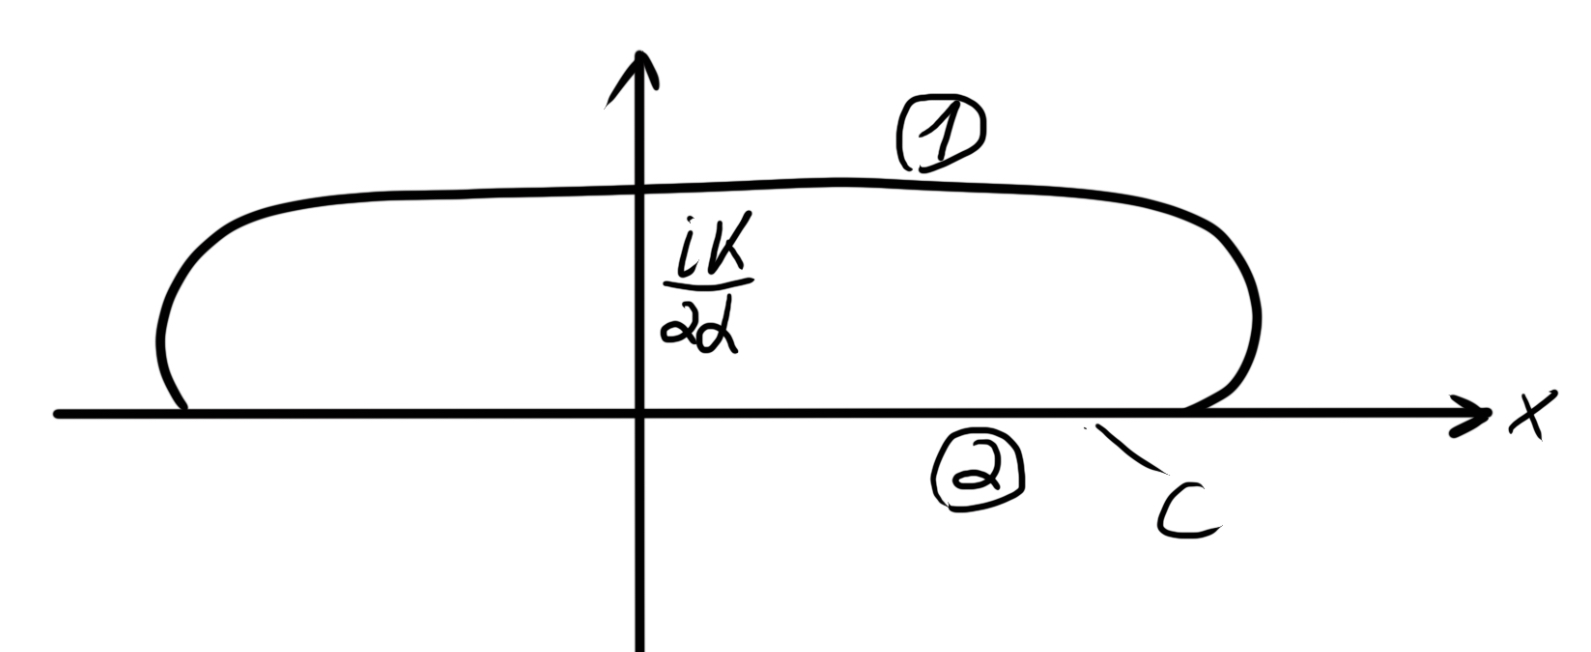
\includegraphics[width=0.5\textwidth]{/Users/vladbelousov/Desktop/Semestr_4-FP-NSU/ДфУ/Лекции_по_дням/image/23.png}
\end{center}

Вопрос: если \( y_0 \approx y_0^* \), можно ли утверждать, что \( y(t, y_0 ^* ) \approx y (t, y_0) \) 

Пример: 

\[ \begin{aligned}
    \begin{aligned}
        &\begin{cases}
            y ' = y ^2  \\ 
            y(0 ) = y^* = 0 
        \end{cases} \\
        &y(t, 0 )=0 , \text{ } t \in (-\infty , +\infty )
    \end{aligned}
    \quad \quad  
    \begin{aligned}
        &\begin{cases}
            y ' = y ^2 \\
            y(0) = y_0 > 0
        \end{cases} \\
        &y(t,y_0) = \frac{1 }{\frac{1}{y_0 } -t } , \text{ } t \in  \left( -\infty , \frac{1}{y_0}  \right)
    \end{aligned}
\end{aligned} \] 

\begin{center}
    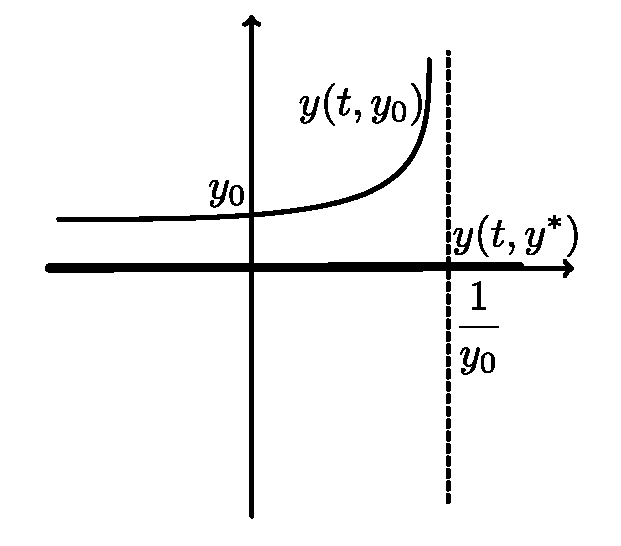
\includegraphics[width=0.4\textwidth]{/Users/vladbelousov/Desktop/Semestr_4-FP-NSU/ДфУ/Лекции_по_дням/image/25.pdf}
\end{center}

\begin{theorem}
    Пусть \( f \in C(\mathbb{D}) , \text{ } \exists \frac{\partial f}{\partial y} \in C(\mathbb{D}) \). Пусть \((t_0, y_0^*) \in \mathbb{D}\). Пусть \( y(t, y_0^*) \) - решение задачи Коши, определенное на интервале \( (\alpha, \omega) \). Возьмем \( [t_1, t_2] \subset (\alpha, \omega) \). Тогда:

    1) \( \exists \Delta > 0 , \text{ }  \forall  y_0 : \left\lvert y_0 - y_0 ^*  \right\rvert < \Delta \Rightarrow y(t, y_0)\)  определенно при \( t \in  [t_1, t_2 ] \); 
    
    2) \( y(t, y_0 ) \xrightarrow{y_0 \to  y_0^* } y(t, y_0^*) , \text{ }  t \in [t_1, t_2 ]  \)
\end{theorem}

Пример: 

\[ (t_0, y_0 ^* ) = (0,0 ) \Rightarrow y (t, y_0 ^* ) \equiv 0 , \text{ } (\alpha , \omega ) = (-\infty , + \infty  ). \text{ Возьмем: } [-T, T]  \] 

\begin{center}
    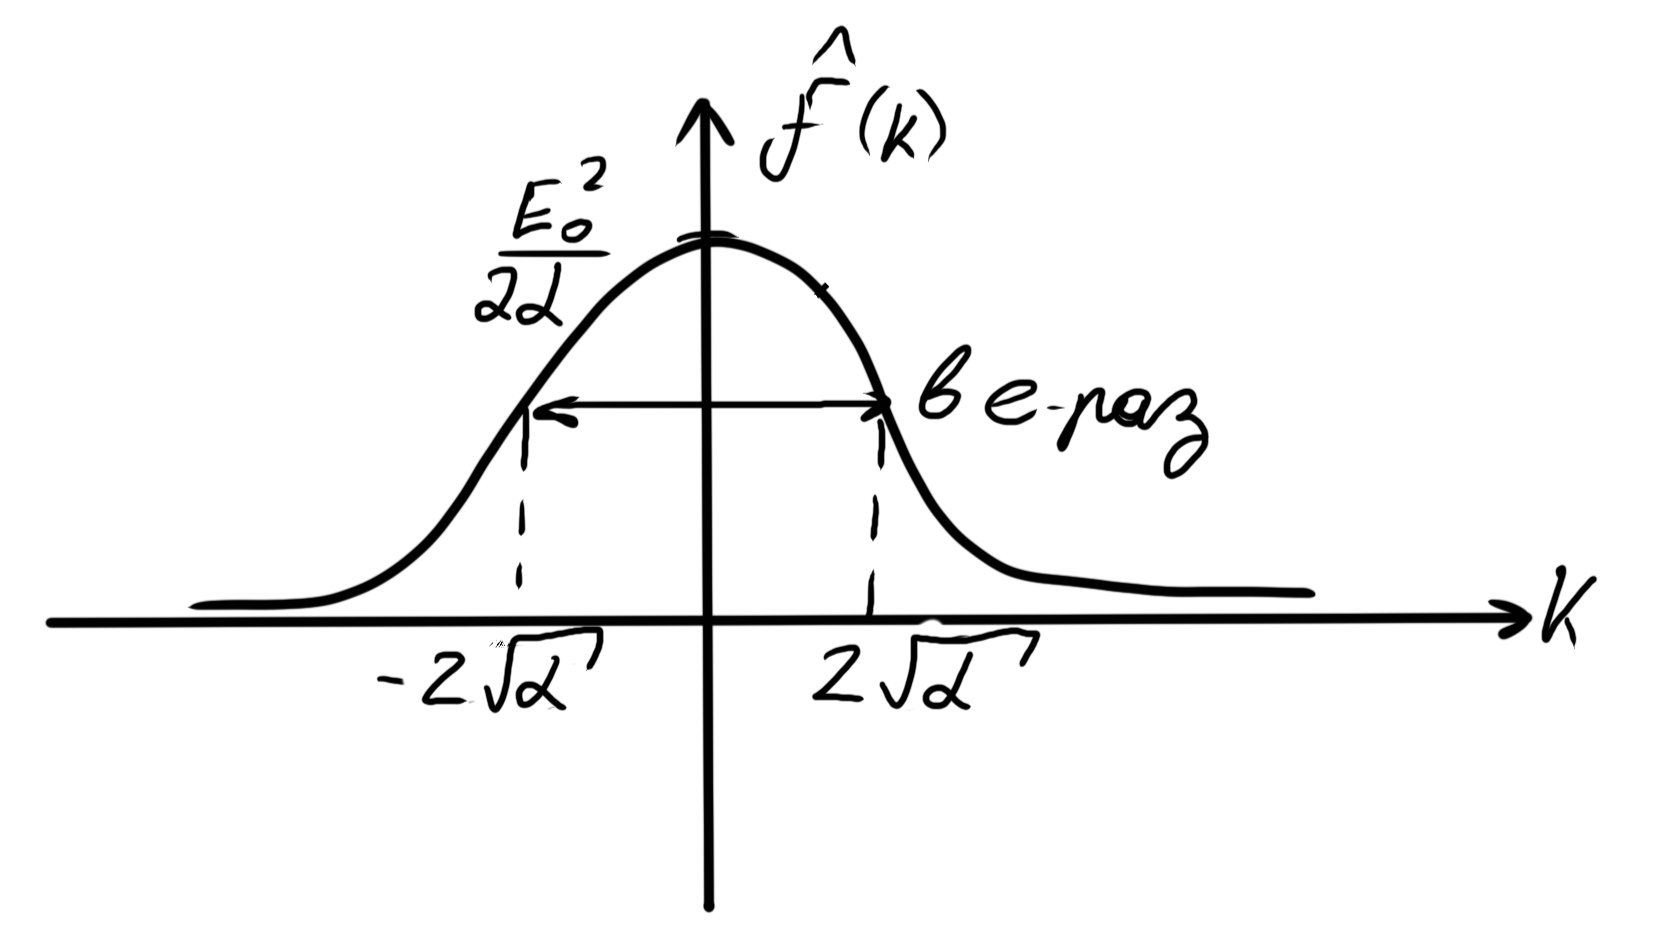
\includegraphics[width=0.4\textwidth]{/Users/vladbelousov/Desktop/Semestr_4-FP-NSU/ДфУ/Лекции_по_дням/image/24.png}
\end{center} 
\[ 1) \text{ } y_0 > 0 ;\text{ }  T < \frac{1}{y_0 } \Leftrightarrow y_0 < \frac{1}{T } =\Delta  \] 

\[ 2) \text{ } y(t,y_0 )= \frac{1}{\frac{1}{y_0 } - t    } \xrightarrow{y_0 \to  0 } 0 , \text{  }  t \in [-T,T]    \] 

%%-------------------------------%%

% Закрытие документа, если файл компилируется отдельно
\ifdefined\mainfile
    % Если это основной файл, не нужно заканчивать документ
\else
    \end{document}
\fi